%\documentclass[UTF8]{ctexart} % use larger type; default would be 10pt
\documentclass[a4paper]{article}
\usepackage{xeCJK}
%\usepackage[utf8]{inputenc} % set input encoding (not needed with XeLaTeX)

%%% Examples of Article customizations
% These packages are optional, depending whether you want the features they provide.
% See the LaTeX Companion or other references for full information.

%%% PAGE DIMENSIONS
\usepackage{geometry} % to change the page dimensions
\geometry{a4paper} % or letterpaper (US) or a5paper or....
\geometry{margin=1in} % for example, change the margins to 2 inches all round
% \geometry{landscape} % set up the page for landscape
%   read geometry.pdf for detailed page layout information

\usepackage{graphicx} % support the \includegraphics command and options

% \usepackage[parfill]{parskip} % Activate to begin paragraphs with an empty line rather than an indent

%%% PACKAGES
\usepackage{booktabs} % for much better looking tables
\usepackage{array} % for better arrays (eg matrices) in maths
\usepackage{paralist} % very flexible & customisable lists (eg. enumerate/itemize, etc.)
\usepackage{verbatim} % adds environment for commenting out blocks of text & for better verbatim
\usepackage{subfig} % make it possible to include more than one captioned figure/table in a single float
% These packages are all incorporated in the memoir class to one degree or another...

%%% HEADERS & FOOTERS
\usepackage{fancyhdr} % This should be set AFTER setting up the page geometry
\pagestyle{fancy} % options: empty , plain , fancy
\renewcommand{\headrulewidth}{0pt} % customise the layout...
\lhead{}\chead{}\rhead{}
\lfoot{}\cfoot{\thepage}\rfoot{}

%%% SECTION TITLE APPEARANCE
\usepackage{sectsty}
\allsectionsfont{\sffamily\mdseries\upshape} % (See the fntguide.pdf for font help)
% (This matches ConTeXt defaults)

%%% ToC (table of contents) APPEARANCE
\usepackage[nottoc,notlof,notlot]{tocbibind} % Put the bibliography in the ToC
\usepackage[titles,subfigure]{tocloft} % Alter the style of the Table of Contents
\renewcommand{\cftsecfont}{\rmfamily\mdseries\upshape}
\renewcommand{\cftsecpagefont}{\rmfamily\mdseries\upshape} % No bold!

%%% END Article customizations

%%% The "real" document content comes below...

\setlength{\parindent}{0pt}
\usepackage{physics}
\usepackage{amsmath}
%\usepackage{symbols}
\usepackage{AMSFonts}
\usepackage{bm}
%\usepackage{eucal}
\usepackage{mathrsfs}
\usepackage{amssymb}
\usepackage{float}
\usepackage{multicol}
\usepackage{abstract}
\usepackage{empheq}
\usepackage{extarrows}
\usepackage{textcomp}
\usepackage{fontspec}
\usepackage{braket}
\usepackage{siunitx}
\sisetup{
	separate-uncertainty = true,
	inter-unit-product = \ensuremath{{}\cdot{}}
}
\usepackage{mhchem}
\usepackage{hyperref}
\hypersetup{
	colorlinks=true,
	linkcolor=black,
	filecolor=magenta,      
	urlcolor=cyan,
}

\DeclareMathOperator{\p}{\prime}
\DeclareMathOperator{\ti}{\times}
\DeclareMathOperator{\intinf}{\int_0^\infty}
\DeclareMathOperator{\intdinf}{\int_{-\infty}^\infty}
\DeclareMathOperator{\intzpi}{\int_0^\pi}
\DeclareMathOperator{\intztpi}{\int_0^{2\pi}}
\DeclareMathOperator{\sumninf}{\sum_{n=1}^{\infty}}
\DeclareMathOperator{\sumninfz}{\sum_{n=0}^\infty}
\DeclareMathOperator{\sumiinf}{\sum_{i=1}^{\infty}}
\DeclareMathOperator{\sumiinfz}{\sum_{i=0}^\infty}
\DeclareMathOperator{\sumkinf}{\sum_{k=1}^{\infty}}
\DeclareMathOperator{\sumkinfz}{\sum_{k=0}^\infty}
\DeclareMathOperator{\e}{\mathrm{e}}
\DeclareMathOperator{\I}{\mathrm{i}}
\DeclareMathOperator{\Arg}{\mathrm{Arg}}
\newcommand{\NA}{N_\mathrm{A}}
\newcommand{\kB}{k_\mathrm{B}}

\DeclareMathOperator{\ra}{\rightarrow}
\DeclareMathOperator{\llra}{\longleftrightarrow}
\DeclareMathOperator{\lra}{\longrightarrow}
\DeclareMathOperator{\dlra}{\Leftrightarrow}
\DeclareMathOperator{\dra}{\Rightarrow}
\newcommand{\bkk}[1]{\Braket{#1|#1}}
\newcommand{\bk}[2]{\Braket{#1|#2}}
\newcommand{\bkev}[2]{\Braket{#2|#1|#2}}



\DeclareMathOperator{\hV}{\hat{\vb{V}}}

\DeclareMathOperator{\hx}{\hat{\vb{x}}}
\DeclareMathOperator{\hy}{\hat{\vb{y}}}
\DeclareMathOperator{\hz}{\hat{\vb{z}}}

\DeclareMathOperator{\hA}{\hat{\vb{A}}}

\DeclareMathOperator{\hQ}{\hat{\vb{Q}}}
\DeclareMathOperator{\hI}{\hat{\vb{I}}}
\DeclareMathOperator{\psis}{\psi^\ast}
\DeclareMathOperator{\Psis}{\Psi^\ast}
\DeclareMathOperator{\hi}{\hat{\vb{i}}}
\DeclareMathOperator{\hj}{\hat{\vb{j}}}
\DeclareMathOperator{\hk}{\hat{\vb{k}}}
\DeclareMathOperator{\hr}{\hat{\vb{r}}}
\DeclareMathOperator{\hT}{\hat{\vb{T}}}
\DeclareMathOperator{\hH}{\hat{H}}
\DeclareMathOperator{\hh}{\hat{h}}               % helicity
\DeclareMathOperator{\hL}{\hat{\vb{L}}}
\DeclareMathOperator{\hp}{\hat{\vb{p}}}

\DeclareMathOperator{\ha}{\hat{\vb{a}}}
\DeclareMathOperator{\hS}{\hat{\vb{S}}}
\DeclareMathOperator{\hSigma}{\hat{\bm\Sigma}}
\DeclareMathOperator{\hJ}{\hat{\vb{J}}}
\DeclareMathOperator{\hP}{\hat{\vb{P}}}          % Parity
\DeclareMathOperator{\hC}{\hat{\vb{C}}} 
\DeclareMathOperator{\Tdv}{-\dfrac{\hbar^2}{2m}\dv[2]{x}}
\DeclareMathOperator{\Tna}{-\dfrac{\hbar^2}{2m}\nabla^2}
\DeclareMathOperator{\vna}{\vnabla}
\DeclareMathOperator{\nna}{\nabla^2}
\newcommand{\naCarExpd}[1]{\pdv[2]{#1}{x} + \pdv[2]{#1}{y} + \pdv[2]{#1}{z}}
\newcommand{\naCyl}{\qty[\dfrac{1}{\rho}\pdv{\rho}\qty(\rho\pdv{\rho}) + \dfrac{1}{\rho^2}\pdv[2]{\phi} + \pdv[2]{z}]}

%\DeclareMathOperator{\g#0}{\gamma^0}
%\DeclareMathOperator{\g1}{\gamma^1}
%\DeclareMathOperator{\g2}{\gamma^2}
%\DeclareMathOperator{\g3}{\gamma^3}
%\DeclareMathOperator{\g5}{\gamma^5}
\newcommand{\g}[1]{\gamma^{#1}}
\DeclareMathOperator{\gmuu}{\gamma^\mu}
\DeclareMathOperator{\gmud}{\gamma_\mu}
%\newcommand{\G}[2]{g^{#1#2}}

\newcommand{\subsbul}{\subsection*{$ \bullet $}}
\newcommand{\ex}[1]{\paragraph{28-#1}}
\newcommand{\subex}[1]{\subparagraph{#1}}
\newcommand{\dis}{\displaystyle}
\newcommand{\iden}{{\large \bm{1}}}
\newcommand{\qed}{$ \Square $}
\newcommand{\tPhi}{\tilde{\Phi} }
\DeclareMathOperator{\au}{\mathrm{a.u.}}
\newcommand{\ntg}{\notag\\}
\DeclareMathOperator{\rms}{\mathrm{rms}}

\numberwithin{equation}{section}
%\setcounter{secnumdepth}{4}
\setcounter{tocdepth}{4}
\allowdisplaybreaks[4]

\usepackage{xcolor}
\definecolor{codegray}{gray}{0.9}
\newfontfamily\Consolas{Consolas}
\newcommand{\code}[1]{\colorbox{codegray}{{\Consolas#1}}}

\title{\textbf{Advanced Physical Chemistry II}\\HW   Part II}
\author{王石嵘
\vspace{5pt}\\
161240065\\
%Email: shirong\_wang@berkeley.edu
}
\date{\today} % Activate to display a given date or no date (if empty),
         % otherwise the current date is printed 

\begin{document}
% \boldmath

\maketitle

%\tableofcontents

%\newpage

\setcounter{section}{27}
\section{The Rate of a Bimolecular Gas-Phase Reaction}
15,18,21,22,23,27,28,29,30,32,33,34,37,43,44\\

\ex{15}
For monatomic gas,
\begin{equation}\label{key}
\gamma = \dfrac{5}{3}
\end{equation}
thus
\begin{equation}\label{key}
u_{\text{peak}}(\ce{He}) = \sqrt{\dfrac{2\times 8.3145\times 300}{0.004003}}\sqrt{\dfrac{5/3}{5/3-1}} = \SI{1765}{m/s}
\end{equation}
\begin{equation}\label{key}
u_{\text{peak}}(\ce{Ne}) = \sqrt{\dfrac{2\times 8.3145\times 300}{0.02018}}\sqrt{\dfrac{5/3}{5/3-1}} = \SI{786.1}{m/s}
\end{equation}

\ex{18}
\subex{$ \bullet $} No vibrational motion:\\
Since 
\begin{equation}\label{key}
\dfrac{1}{2}\mu u_r^2(R) = E_{\text{int}}(P) + \dfrac{1}{2}\mu u_r^2(P) -  E_{\text{int}}(R) \geq E_{\text{int}}(P)  -  E_{\text{int}}(R) 
\end{equation}
we have
\begin{align}
u_{r,min} &= \sqrt{\dfrac{2 (E_{\text{int}}(P)  -  E_{\text{int}}(R) )}{\mu}} \notag\\
&= \sqrt{\dfrac{2\times 12400}{\dfrac{35.453\times 2.016}{35.453+2.016}\times 10^{-3}}} \notag\\
&= \SI{3606}{m/s}
\end{align}
\subex{$ \bullet $} Hard-sphere harmonic oscillators:\\
\begin{align}\label{key}
\dfrac{1}{2}\mu u_r^2(R) &\geq E_{\text{int}}(P)  -  E_{\text{int}}(R) = D_e(\ce{H_2}) - D_e(\ce{HCl}) + E_{\text{vib}}(P) - E_{\text{vib}}(R) \notag\\
&= \SI{12.4}{kJ/mol} + hc\NA(\SI{2886}{cm^{-1}} - \SI{4159}{cm^{-1}})\dfrac{1}{2} \notag\\
&= \SI{4.79}{kJ/mol}
\end{align}
thus
\begin{align}
u_{r,min} %&= \sqrt{\dfrac{2 (E_{\text{int}}(P)  -  E_{\text{int}}(R) )}{\mu}} \notag\\
&= \sqrt{\dfrac{2\times 47900}{\dfrac{35.453\times 2.016}{35.453+2.016}\times 10^{-3}}} \notag\\
&= \SI{2241}{m/s}
\end{align}

\ex{21}
\begin{align}
\dfrac{1}{2}\mu u_r^2(P) &= \dfrac{1}{2}\mu u_r^2(R) + E_{\text{vib}}(R) - E_{\text{vib}}(P) + D_e(\ce{DF}) - D_e(\ce{D_2}) \notag\\
&= \SI{7.62}{kJ/mol} + \dfrac{1}{2}hc\NA(2990-2907)\si{cm^{-1}} + \SI{140}{kJ/mol} \notag\\
&= \SI{148}{kJ/mol}
\end{align}
thus
\begin{equation}\label{key}
u_r(P) = \sqrt{\dfrac{2\times \num{148e3}}{\num{3.05e-27}}} = \SI{1.27e4}{m/s}
\end{equation}
thus $ \abs{\vb{u}_{\ce{DF}} - \vb{u}_{cm}}, \abs{\vb{u}_{\ce{D}} - \vb{u}_{cm}}  $ remains the same as Example 28-5, as follows
\begin{equation}\label{key}
\abs{\vb{u}_{\ce{DF}} - \vb{u}_{cm}} = \dfrac{m_{\ce{D}}}{M}u_r(P) = \SI{1.16e3}{m/s}
\end{equation}
\begin{equation}\label{key}
\abs{\vb{u}_{\ce{D}} - \vb{u}_{cm}} = \dfrac{m_{\ce{DF}}}{M}u_r(P) = \SI{1.21e4}{m/s}
\end{equation}


\ex{22}
\begin{equation}\label{key}
E_{\text{vib}} = \tilde{\nu}_e(1/2) - \tilde{x}_e\tilde{\nu}_e(1/2)^2 = \SI{1313.2}{cm^{-1}} = \SI{15.71}{kJ/mol}
\end{equation}
$ \therefore $
\begin{equation}\label{key}
E_{\text{trans}}' = E_{\text{trans}} + E_{\text{vib}} - E_{\text{vib}}' - [ D_e(\ce{HBr}) - D_e(\ce{HCl})] > 0
\end{equation}
\begin{equation}\label{key}
9.21 + 15.71 - E_{\text{vib}}' + 67.2 > 0
\end{equation}
\begin{equation}\label{key}
E_{\text{vib}}' < \SI{92.12}{kJ/mol} = \SI{7701.2}{cm^{-1}}
\end{equation}
$ \therefore $
\begin{equation}\label{key}
2990.95 (v + 1/2) - 52.82 (v+1/2)^2 < 7701.2
\end{equation}
\begin{equation}\label{key}
v < 2.20 
\end{equation}
i.e. $ v=0,1,2 $\\
The energy diagram is as follows
\begin{figure}[H]
	\centering
	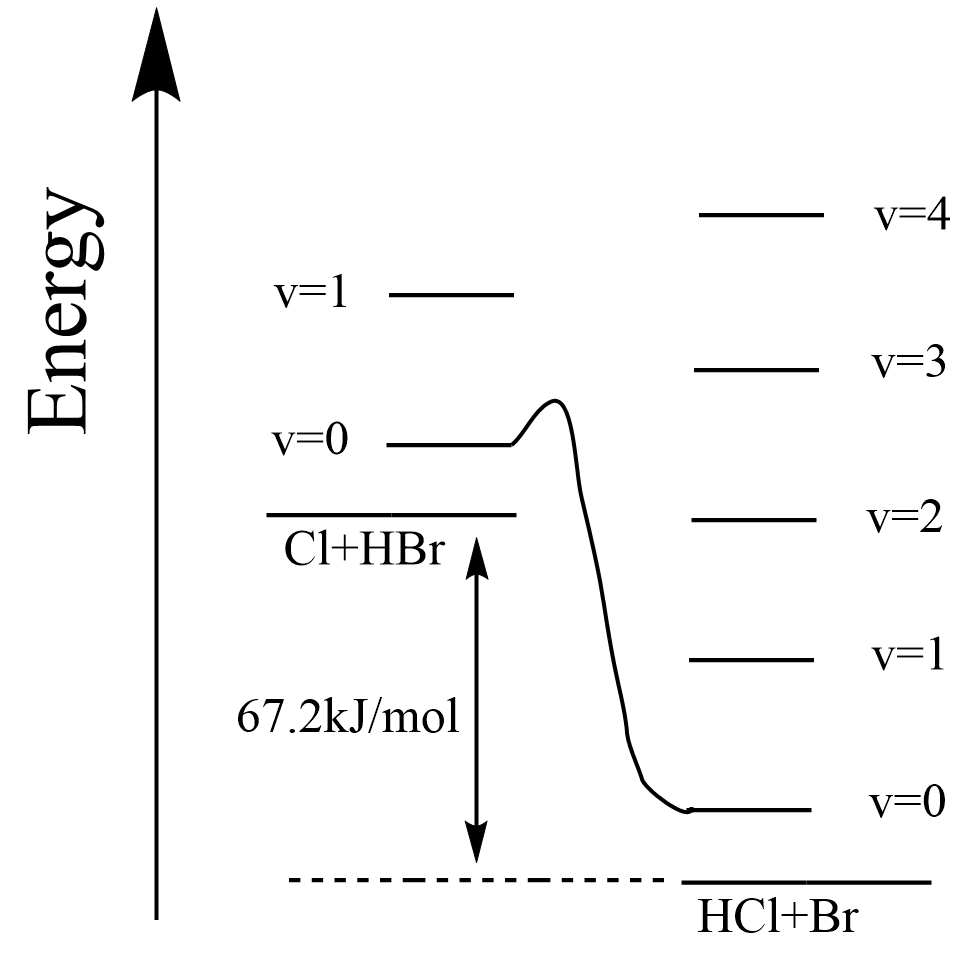
\includegraphics[width=0.5\linewidth]{28-22.png}
\end{figure}

\ex{23}
From 28-22, we have
\begin{equation}\label{key}
E_{\text{trans}}' = E_{\text{trans}} + E_{\text{vib}} - E_{\text{vib}}' - [ D_e(\ce{HBr}) - D_e(\ce{HCl})] = \SI{92.12}{kJ/mol} - E_{\text{vib}}' 
\end{equation}
thus
\begin{align}\label{key}
u_r' &= \sqrt{\dfrac{2[92120 - \tilde{\nu}_e(v+1/2) + \tilde{\nu}_e\tilde{x}_e(v+1/2)^2}{\mu'}} \notag\\
&= \sqrt{\dfrac{2[92120 - 35772(v+1/2) + 631.7(v+1/2)^2}{\num{2.504e-2}}} \si{m/s}
\end{align}
\begin{align}
\abs{\vb{u}_{\ce{HCl}} - \vb{u}_{cm}} &= \dfrac{m_{\ce{Br}}}{M}u_r' \notag\\
&= \dfrac{79.904}{116.365}u_r' = 0.68667u_r' 
\end{align}
$ \therefore $
\begin{table}[H]
	\centering
	\begin{tabular}{ccc}
		\hline
		$ v $ & $ u_r' \;/\; \si{m/s} $ & $ \abs{\vb{u}_{\ce{HCl}} - \vb{u}_{cm}} \;/\; \si{m/s} $ \\ \hline
		0 & 2438 & 1674 \\
		1 & 1785 & 1226 \\
		2 & 728.1 & 500.0\\ \hline
	\end{tabular}
\end{table}


\ex{27}
They will increase.\\
Since $ u_r \propto \sqrt{E_{\text{trans}}} $, the radius will increase by $ \sqrt{2} $.


\ex{28}
\begin{align}
E_{\text{rot}}' &= \tilde{\nu}_e\qty(\dfrac{7}{2}-\dfrac{5}{2}) - \tilde{\nu}_e\tilde{x}_e\qty[\qty(\dfrac{7}{2})^2 - \qty(\dfrac{5}{2})^2] \notag\\
&= 2998.3\times 1 - 45.71\times 6 \si{cm^{-1}}\notag\\
&=  \SI{2724.0}{cm^{-1}}
\end{align}
while
\begin{equation}\label{key}
E_{\text{rot}}' =  [\tilde{B}_e - \tilde\alpha_e(v+1/2)]J(J+1)
\end{equation}
we have
\begin{equation}\label{key}
2724.0 = [11.007 - 0.293\times (5/2)] J(J+1)
\end{equation}
\begin{equation}\label{key}
J = 15.8 \approx 16
\end{equation}
which is too large, so there could not be a problem encountered in the analysis of the scatttering data.


\ex{29}
\begin{equation}\label{key}
E_{vib} = \tilde{\nu}_e(v+1/2) - \tilde{\nu}_e\tilde{x}_e(v+1/2)^2 = \SI{13917.82}{cm^{-1}}
\end{equation}
\begin{equation}\label{key}
E_{\text{trans}}' = E_{\text{trans}} + E_{\text{vib}} - [D_e(\ce{H_2})-D_e(\ce{HCl})] > 0
\end{equation}
$ \therefore $
\begin{equation}\label{key}
703.91 + 13917.82 - 1036.64   - E_{\text{vib}}' > 0 
\end{equation}
\begin{equation}\label{key}
2990.95(v+1/2) - 52.82(v+1/2)^2 < 13585.90
\end{equation}
\begin{equation}\label{key}
v < 4.5
\end{equation}
thus $ v = 0,1,2,3,4 $.

\ex{30}
From 28-29, we have
\begin{equation}\label{key}
2990.95(4+1/2) - 52.82(4+1/2)^2 + [\tilde{B}_e - \tilde\alpha_e(4+1/2)]J(J+1) < 13585.90
\end{equation}
\begin{equation}\label{key}
2990.95(4+1/2) - 52.82(4+1/2)^2 + [10.59 - 0.307(4+1/2)]J(J+1) < 13585.90
\end{equation}
\begin{equation}\label{key}
J < 10.9
\end{equation}
thus $ J_{max} = 10 $.

\ex{32}
stripping, because the scattering is localized in the forward direction.


\ex{33}
More low relative velocity products in (b) have internal energy that are greater than $ D_e(\ce{N_2D^+}) $. 


\ex{34}
\begin{equation}\label{key}
\sigma = \pi\qty(\dfrac{200 + 740}{2})^2 = \SI{6.94e5}{pm^2}
\end{equation}
which is smaller than the measured cross section, which means a harpoon mechanism.


\ex{37}
The PES is 4-dimensional for the first reaction, and 9-dimensional for the second.


%\ex{43}



%\ex{44}


%\ex{extra}



\end{document}